\documentclass[12pt,a4paper,oneside]{report}

\usepackage[a4paper,top=2.5cm,bottom=2.5cm,left=3cm,right=2.5cm]{geometry}
\usepackage{fontspec}
\setmainfont{Times New Roman}
\usepackage[french]{babel}
\usepackage{csquotes}
\usepackage{setspace}
\onehalfspacing
\usepackage{microtype}
\usepackage{graphicx}
\usepackage{booktabs}
\usepackage{longtable}
\usepackage{array}
\usepackage{float}
\usepackage{caption}
\usepackage{xcolor}
\usepackage{hyperref}
\usepackage[backend=biber,style=authoryear,sorting=nyt,maxcitenames=2,maxbibnames=20]{biblatex}
\addbibresource{references.bib}

\definecolor{accent}{HTML}{287271}
\hypersetup{colorlinks=true,linkcolor=accent,citecolor=accent,urlcolor=accent,pdftitle={Quel est l'impact de l'IA dans les processus de développement logiciel ?},pdfauthor={Baptiste Cariat}}
\captionsetup{font=small,labelfont=bf}
\setlength{\parindent}{1.1cm}
\setlength{\parskip}{0.2em}
\renewcommand{\arraystretch}{1.2}

\newcommand{\taux}[1]{#1\,\%}
\newcommand{\ia}{intelligence artificielle}

\begin{document}

\begin{titlepage}
  \centering
  {\large Institut national universitaire Champollion\par}
  \vspace{0.5cm}
  {\large Master 2 AMINJ\par}
  {\normalsize Audiovisuel, Multimédia Interactif, Numérique, Jeux\par}
  \vfill
  {\Huge\bfseries Quel est l'impact de l'intelligence artificielle dans les processus de développement logiciel ?\par}
  \vspace{1cm}
  {\Large Mémoire de Master 2\par}
  \vfill
  {\Large Baptiste Cariat\par}
  \vspace{1.5cm}
  \begin{tabular}{rl}
    Encadrant : & Michel Galaup \\
    Année universitaire : & 2025--2026
  \end{tabular}
  \vfill
\end{titlepage}

\pagenumbering{roman}

\chapter*{Résumé}
\addcontentsline{toc}{chapter}{Résumé}
L'intelligence artificielle générative est désormais présente dans les environnements de développement et les outils de revue. Certains agents peuvent même produire des modifications à l'échelle d'un dépôt. Ces outils promettent des gains de productivité, mais posent aussi des questions de qualité, de sécurité et de responsabilité. Ce mémoire étudie leurs effets à partir de travaux scientifiques et de traces publiques issues de Git et GitHub.

L'état de l'art montre que l'effet sur la vitesse dépend fortement du contexte. Une expérience contrôlée rapporte une réduction de temps de \taux{55,8} sur une tâche courte, une étude en entreprise estime ce gain à environ \taux{21}, tandis qu'une expérience menée auprès de mainteneurs expérimentés observe au contraire un ralentissement de \taux{19}. Les travaux sur la qualité et la sécurité montrent également que la production de code fonctionnel ne garantit ni sa maintenabilité ni son innocuité.

L'expérimentation porte sur six dépôts principaux et deux dépôts complémentaires entre juin 2020 et août 2026. Elle recherche uniquement des mentions explicites d'un outil d'IA dans les commits et les pull requests. Sur les six dépôts principaux, 7\,303 commits sur 282\,415 et 3\,186 pull requests sur 220\,460 contiennent une telle mention. Dans les trois projets où une date d'adoption a pu être identifiée, les taux augmentent nettement après cette date. Ces chiffres montrent que les agents deviennent plus visibles dans le processus de développement. Ils ne permettent cependant d'estimer ni la part de code réellement écrite par IA ni son effet sur la qualité.

L'impact de l'IA varie selon la tâche, l'expérience du développeur et le projet. Elle modifie surtout la répartition du travail entre la formulation d'une demande, la génération d'une solution, sa vérification et son intégration. Dans un cadre professionnel, les tests, la revue et la traçabilité restent donc indispensables.

\noindent\textbf{Mots-clés :} intelligence artificielle générative, développement logiciel, productivité, qualité du code, sécurité, GitHub, agents de développement.

\tableofcontents
\clearpage
\pagenumbering{arabic}

\chapter{Introduction}

La génération de code assistée par intelligence artificielle a quitté le seul cadre de la recherche. Des outils comme GitHub Copilot, Cursor, Claude Code ou Codex peuvent compléter une fonction, expliquer une base de code, générer des tests et parfois produire une pull request complète. Ils interviennent donc dans plusieurs étapes du travail, depuis la formulation de la tâche jusqu'à la soumission d'une solution à l'équipe.

Le nombre de lignes générées ne suffit pas à mesurer cette évolution. Développer un logiciel demande aussi de comprendre un besoin, de concevoir une solution, de la tester, de la relire et de la maintenir. Le temps gagné pendant l'écriture peut être perdu lors de la vérification. Une suggestion imparfaite peut néanmoins être utile si elle permet d'explorer rapidement plusieurs pistes. \textcite{forsgren2021space} rappellent ainsi que la productivité ne se réduit pas au volume produit : elle dépend également de la satisfaction, de la performance, de la communication et de l'efficacité.

La question centrale de ce mémoire est donc la suivante :

\begin{quote}
\centering\bfseries
Quel est l'impact de l'intelligence artificielle dans les processus de développement logiciel ?
\end{quote}

Pour rendre cette question analysable, je la décline en quatre sous-questions :
\begin{enumerate}
  \item Dans quelles conditions l'assistance par IA accélère-t-elle ou ralentit-elle le travail de développement ?
  \item Quels effets observe-t-on sur la qualité, la maintenabilité et la sécurité du code ?
  \item Comment l'IA transforme-t-elle la répartition du travail entre production, vérification et collaboration ?
  \item Comment cette transformation devient-elle visible dans les traces publiques des dépôts logiciels ?
\end{enumerate}

Pour répondre à ces questions, je m'appuie d'abord sur des expériences contrôlées, des études de terrain et des observations d'utilisateurs. J'analyse ensuite huit dépôts publics à la recherche de traces explicites laissées dans Git et GitHub : compte d'agent, branche dédiée ou déclaration dans une pull request. Je ne cherche pas à deviner l'origine d'un code à partir de son style.

Le chapitre 1 définit les concepts et précise le périmètre. Le chapitre 2 présente l'état de l'art selon une approche à la fois chronologique, thématique et méthodologique. Le chapitre 3 décrit le protocole empirique. Le chapitre 4 expose les résultats. Enfin, le chapitre 5 confronte ces résultats à la littérature et discute leurs limites.

\chapter{Cadre conceptuel et problématisation}

\section{Définir l'intelligence artificielle}

Selon la définition actualisée de l'OCDE, un système d'IA est un système fondé sur une machine qui infère, à partir des données reçues, la manière de produire des prédictions, du contenu, des recommandations ou des décisions \parencite{oecd2024definition}. Cette définition ne renvoie pas à une technique particulière. Elle permet aussi d'inclure des systèmes dont le degré d'autonomie varie.

Le NIST traite l'IA générative comme une classe de systèmes capables de produire du contenu synthétique dérivé de la structure de leurs données d'entrée \parencite{nist2024genai}. Dans le développement logiciel, ce contenu peut être du code, des tests, de la documentation, une explication, une proposition de correction ou un plan d'action. Les assistants étudiés reposent principalement sur de grands modèles de langage entraînés sur du texte et du code. Ils prédisent une suite plausible à partir du contexte fourni ; ils ne garantissent ni l'exactitude fonctionnelle, ni la sécurité, ni l'adéquation aux conventions d'un projet.

\section{Définir le processus de développement logiciel}

Dans ce mémoire, le processus de développement désigne l'ensemble des activités qui transforment un besoin en modification intégrée et maintenue : analyse, conception, implémentation, test, revue, déploiement et maintenance. Les traces étudiées se concentrent sur deux objets observables : le commit et la pull request. Le commit matérialise une modification versionnée. La pull request ajoute une dimension collective : elle rassemble une proposition, une description, des échanges, des contrôles automatiques et une décision d'intégration.

L'IA intervient désormais à plusieurs de ces étapes : elle génère une première implémentation, reformule une exigence, propose des tests ou explique un échec de compilation. Les agents récents peuvent aussi parcourir un dépôt, modifier plusieurs fichiers et soumettre une branche. L'étude doit donc dépasser la qualité d'une suggestion isolée et considérer l'ensemble du travail qui mène à son intégration.

\section{Hypothèses de travail}

À partir de ces éléments, je formule trois hypothèses :
\begin{description}
  \item[H1 --- Effet conditionnel.] L'IA accélère surtout les tâches bien spécifiées et localisées ; son bénéfice diminue lorsque la tâche exige une compréhension profonde d'un dépôt mature.
  \item[H2 --- Déplacement de l'effort.] L'IA réduit une partie du coût de production, mais déplace l'effort vers la formulation, la sélection, la vérification et la revue.
  \item[H3 --- Visibilité hétérogène.] L'adoption devient visible dans les traces de développement, mais cette visibilité dépend des conventions d'outils et des politiques de chaque dépôt. Une absence de signal ne signifie donc pas une absence d'usage.
\end{description}

Ces hypothèses servent de fil conducteur à l'analyse. La présence d'un outil ne sera jamais considérée, à elle seule, comme la preuve d'une amélioration.

\chapter{État de l'art}

\section{Méthode de recherche bibliographique}

L'état de l'art repose sur une revue narrative de travaux consacrés aux assistants de programmation. J'ai retenu en priorité les expériences contrôlées, les études sur les interactions entre humains et IA, les analyses de sécurité et les synthèses récentes. Cette sélection ne constitue pas une revue systématique exhaustive, mais elle permet de confronter plusieurs méthodes et plusieurs contextes d'usage.

La revue systématique de \textcite{hou2024slr} analyse 395 publications parues entre janvier 2017 et janvier 2024. Elle donne une vue d'ensemble des applications des grands modèles de langage en génie logiciel, mais souligne que beaucoup de résultats reposent encore sur des évaluations standardisées. Je l'ai complétée par des travaux consacrés à l'utilisation des assistants, en situation contrôlée ou dans un cadre professionnel.

\section{Une évolution vers l'assistance intégrée et les agents}

Les premiers travaux récents se concentrent sur la complétion de code au sein de l'éditeur. Le développeur conserve l'initiative et accepte ou rejette une proposition locale. Avec les interfaces conversationnelles, il peut ensuite demander une explication, une correction ou une génération à partir d'une consigne en langue naturelle. Les agents actuels franchissent une étape supplémentaire : ils explorent le dépôt, planifient des modifications, exécutent parfois des outils et produisent une branche ou une pull request.

Une fonction générée peut être évaluée avec des tests unitaires. Une modification qui touche plusieurs fichiers demande aussi de vérifier l'architecture, les conventions du projet et le déroulement de la revue. L'attribution devient alors plus difficile : un développeur peut reprendre une suggestion sans laisser de trace, tandis qu'un agent autonome peut utiliser un compte, une branche ou une signature explicite.

\section{Productivité : des résultats dépendants du contexte}

\textcite{peng2023productivity} ont mené une expérience contrôlée dans laquelle des développeurs devaient implémenter un serveur HTTP en JavaScript. Le groupe disposant de GitHub Copilot a terminé la tâche \taux{55,8} plus rapidement que le groupe témoin. L'assistant s'est donc montré efficace pour cette tâche courte et précisément définie. La situation est différente dans un dépôt ancien, où il faut comprendre un contexte plus large et de nombreuses contraintes implicites.

Une expérience menée auprès de 96 ingénieurs de Google par \textcite{paradis2024enterprise} apporte un contexte plus proche de l'entreprise. Les auteurs estiment une réduction d'environ \taux{21} du temps consacré à une tâche complexe avec trois fonctions d'assistance, mais indiquent un intervalle de confiance large et préviennent que le résultat ne se généralise pas automatiquement à d'autres outils ou organisations.

\textcite{becker2025productivity} obtiennent un résultat différent. Seize développeurs expérimentés ont réalisé 246 tâches tirées de projets open source auxquels ils contribuaient depuis cinq ans en moyenne. Les tâches étaient attribuées aléatoirement avec ou sans outils d'IA. Les participants pensaient gagner du temps, mais l'accès à l'IA a finalement augmenté la durée de réalisation de \taux{19}. Dans ce cas, la connaissance du dépôt, les exigences de qualité et le temps consacré au contrôle ont annulé le gain attendu.

Ces études portent sur des situations très différentes : une tâche JavaScript isolée, un environnement d'entreprise et des dépôts matures connus de leurs mainteneurs. Leurs résultats confortent H1 : le gain dépend moins de l'outil seul que de la tâche, de l'utilisateur et du contexte.

\section{Interaction, compréhension et déplacement de l'effort}

\textcite{vaithilingam2022expectation} ont comparé les attentes et l'expérience d'utilisateurs de générateurs de code. Leur étude met en évidence une difficulté centrale : une proposition plausible est rapide à produire mais parfois coûteuse à comprendre et à corriger. L'assistance peut donc améliorer la vitesse perçue sans réduire proportionnellement l'effort global.

À partir de l'observation de vingt participants, \textcite{barke2023grounded} distinguent deux modes d'interaction. Dans le premier, le développeur sait déjà ce qu'il veut produire et utilise le modèle pour aller plus vite. Dans le second, il s'appuie sur les suggestions pour explorer des solutions. L'outil n'a donc pas le même rôle selon que l'utilisateur possède déjà une idée précise de la solution ou qu'il cherche encore une piste.

Une partie du travail se déplace ainsi de l'écriture vers la formulation, la sélection et la validation. L'expertise reste essentielle : plus une suggestion est facile à produire, plus il faut savoir repérer une erreur subtile. La revue de code et les tests prennent alors davantage de place dans le processus.

\section{Qualité et maintenabilité}

\textcite{dakhel2023asset} comparent les propositions de Copilot à des solutions humaines sur des problèmes de programmation. L'outil fournit des solutions correctes et variées, mais produit aussi des erreurs qui nécessitent une supervision. Son utilité dépend donc en partie de la capacité du développeur à évaluer ce qu'il propose.

L'étude de \textcite{yetistiren2023quality} évalue GitHub Copilot, Amazon CodeWhisperer et ChatGPT sur HumanEval selon plusieurs dimensions. Pour les versions étudiées, les taux de solutions correctes sont respectivement de \taux{46,3}, \taux{31,1} et \taux{65,2}. Les auteurs relèvent aussi des différences de dette technique estimée. HumanEval porte sur des fonctions courtes et les outils évoluent rapidement : ces chiffres n'établissent donc pas une hiérarchie durable. Ils rappellent surtout qu'un code syntaxiquement valide n'est pas nécessairement correct, maintenable ou sûr.

Le nombre de lignes générées ou le taux d'acceptation des suggestions ne suffisent donc pas à évaluer la qualité. Il faut aussi examiner les tests, les résultats de l'analyse statique, la revue humaine et le devenir du code dans le temps.

\section{Sécurité et gestion des risques}

\textcite{pearce2022security} ont soumis Copilot à des scénarios de programmation sensibles à la sécurité. Leur analyse montre qu'une part substantielle des propositions peut contenir des faiblesses. L'étude porte sur des scénarios contrôlés et sur une version ancienne de l'outil, mais elle établit qu'un code plausible et compilable peut rester vulnérable.

\textcite{perry2023insecure} s'intéressent plutôt au comportement de l'utilisateur. Dans leur étude, certains participants produisent un code moins sûr avec l'assistance, tout en ayant davantage confiance dans leur solution. La facilité avec laquelle une réponse est obtenue peut donc réduire la vigilance.

\textcite{fu2025weaknesses} analysent pour leur part 733 extraits attribués à des générateurs dans des projets GitHub. Ils détectent des faiblesses dans \taux{29,5} des extraits Python et \taux{24,2} des extraits JavaScript, réparties dans 43 catégories CWE. Le corpus provient de projets réels, mais l'attribution des extraits et les résultats de l'analyse statique gardent une part d'incertitude.

Le NIST recommande de prendre en compte les risques de l'IA générative pendant tout le cycle de vie \parencite{nist2024genai}. Dans une équipe logicielle, cela passe notamment par une validation humaine, des tests automatiques, une analyse de sécurité et des règles claires sur les données et la traçabilité.

\section{Synthèse critique des méthodologies}

\small
\begin{longtable}{@{}>{\raggedright\arraybackslash}p{2.9cm}>{\raggedright\arraybackslash}p{3.1cm}>{\raggedright\arraybackslash}p{3.5cm}>{\raggedright\arraybackslash}p{4cm}@{}}
\caption{Principaux travaux mobilisés et portée de leurs résultats.}\label{tab:literature}\\
\toprule
Travail & Méthode & Résultat principal & Limite principale \\
\midrule
\endfirsthead
\toprule
Travail & Méthode & Résultat principal & Limite principale \\
\midrule
\endhead
\textcite{peng2023productivity} & Expérience contrôlée, tâche JavaScript & Réalisation \taux{55,8} plus rapide avec Copilot & Tâche courte et isolée \\
\textcite{paradis2024enterprise} & Essai randomisé, 96 ingénieurs & Gain estimé d'environ \taux{21} & Outillage interne et intervalle large \\
\textcite{becker2025productivity} & Essai randomisé, 246 tâches réelles & Ralentissement de \taux{19} & 16 mainteneurs et projets matures \\
\textcite{barke2023grounded} & Observation qualitative, 20 participants & Modes accélération et exploration & Généralisation statistique limitée \\
\textcite{yetistiren2023quality} & Benchmark HumanEval & Qualité variable selon outils et métriques & Fonctions courtes, versions vite obsolètes \\
\textcite{perry2023insecure} & Étude utilisateur de sécurité & Interaction entre aide, erreurs et confiance & Tâches de sécurité contrôlées \\
\textcite{fu2025weaknesses} & Analyse de 733 extraits GitHub & Faiblesses détectées en Python et JavaScript & Attribution et analyse statique imparfaites \\
\bottomrule
\end{longtable}
\normalsize

\chapter{Méthodologie empirique}

\section{Positionnement de l'étude}

L'étude est quantitative et longitudinale. Elle s'appuie sur les traces publiques laissées au cours du développement. Je ne cherche pas à deviner si un code a été généré à partir de son style, car cette méthode serait difficile à contrôler. Je retiens uniquement des attributions observables de l'intervention d'un outil.

L'unité d'analyse est soit un commit, soit une pull request. Ces deux canaux restent séparés : un commit matérialise une modification, tandis qu'une pull request représente une proposition soumise au processus collectif d'intégration.

\section{Corpus}

Le corpus couvre la période du 1\textsuperscript{er} juin 2020 au 25 août 2026. L'échantillon principal comprend six dépôts : Microsoft VS Code, Home Assistant Core, Next.js, Godot, Redis et Django. Pour les trois premiers, j'ai pu dater l'ajout d'un fichier de configuration destiné à un assistant. Godot, Redis et Django servent de points de comparaison, sans date d'adoption retenue. Le dépôt Django contient même une instruction de rejet de Copilot ; je ne l'ai donc pas classé parmi les projets adoptants.

J'ai ajouté osu! et Bun pour élargir l'observation. Ces deux dépôts restent séparés des comparaisons avant/après. Au total, l'analyse porte sur 347\,168 commits et 246\,767 pull requests.

\section{Détection des attributions explicites}

Le détecteur applique des règles déterministes. Pour les commits, il recherche notamment des identités dédiées et des signatures telles que \texttt{Co-Authored-By} ou \texttt{Generated with Claude Code}. Pour les pull requests, il examine successivement :
\begin{enumerate}
  \item les comptes d'agents et les identités de committer connues ;
  \item les conventions de branche, par exemple \texttt{codex/}, \texttt{cursor/} ou \texttt{copilot/} ;
  \item les liens de tâche et les auto-déclarations strictes dans le titre ou le corps.
\end{enumerate}

Un bot inconnu n'est pas classé comme IA, et le vocabulaire du code n'entre pas dans la décision. La version V2 reprend les règles de la V1 et ajoute les URL de tâches Cursor et Codex, ainsi que de nouvelles formulations explicites. Je l'ai testée sur les 246\,767 pull requests des huit dépôts : elle en détecte 3\,412, contre 3\,406 pour la V1, sans perdre aucun cas déjà repéré.

\section{Mesures et analyses}

Pour chaque dépôt et chaque trimestre, le taux d'attribution est défini par :
\[
Taux_{d,t}=\frac{N_{IA,d,t}}{N_{total,d,t}}\times 100.
\]

La courbe globale représente la moyenne arithmétique des taux des huit dépôts. Ce choix donne le même poids à chaque projet et évite que les dépôts les plus volumineux dominent entièrement la tendance.

Pour les trois dépôts adoptants, les trimestres sont séparés avant et après la date de bascule. Le test de Mann--Whitney compare les distributions trimestrielles sans supposer leur normalité. Une taille d'effet rang-bisériale complète la valeur de $p$. Ces comparaisons restent associatives : la date de bascule n'est pas assignée aléatoirement et d'autres évolutions temporelles peuvent expliquer une partie des écarts.

\section{Validation et limites du dispositif}

Le détecteur V2 est évalué sur AIDev, un corpus de 2\,743\,854 pull requests positives associées à des agents \parencite{aidev2026}. Il en retrouve 2\,611\,681, soit un rappel de \taux{95,18}. Ce corpus ne contient pas un échantillon représentatif de négatifs humains ; il ne permet donc pas d'estimer la précision.

Un développeur peut utiliser un assistant puis intégrer manuellement sa réponse, sans laisser de signal explicite. À l'inverse, une branche portant le nom d'un outil fournit un indice moins solide qu'un compte dédié. Les taux présentés ici sont donc une estimation minimale de l'usage visible, et non une mesure de tout le code généré.

\chapter{Résultats}

\section{Résultats descriptifs}

L'échantillon principal contient 282\,415 commits, dont 7\,303 avec attribution explicite à l'IA, soit \taux{2,59}. Il comprend également 220\,460 pull requests, dont 3\,186 détectées, soit \taux{1,45}. Les deux dépôts exploratoires ajoutent 64\,753 commits et 26\,307 pull requests.

\begin{table}[H]
\centering
\caption{Attributions explicites dans les huit dépôts.}
\label{tab:repos}
\small
\begin{tabular}{lrrrr}
\toprule
Dépôt & Commits & Commits IA & PR & PR IA \\
\midrule
Microsoft VS Code & 97\,341 & 4\,974 & 54\,888 & 2\,458 \\
Home Assistant Core & 88\,323 & 2\,155 & 83\,434 & 358 \\
Next.js & 29\,257 & 148 & 31\,682 & 321 \\
Godot & 57\,203 & 1 & 37\,507 & 18 \\
Redis & 3\,868 & 22 & 4\,670 & 16 \\
Django & 6\,423 & 3 & 8\,279 & 15 \\
osu! & 47\,207 & 0 & 10\,077 & 0 \\
Bun & 17\,546 & 693 & 16\,230 & 226 \\
\bottomrule
\end{tabular}
\end{table}

Les écarts entre projets sont importants. VS Code atteint \taux{5,11} sur les commits et \taux{4,48} sur les pull requests. À l'opposé, aucun signal n'est détecté dans osu!. Cette hétérogénéité peut refléter une différence d'usage, mais aussi des conventions d'attribution et des politiques de contribution différentes.

\begin{figure}[H]
\centering
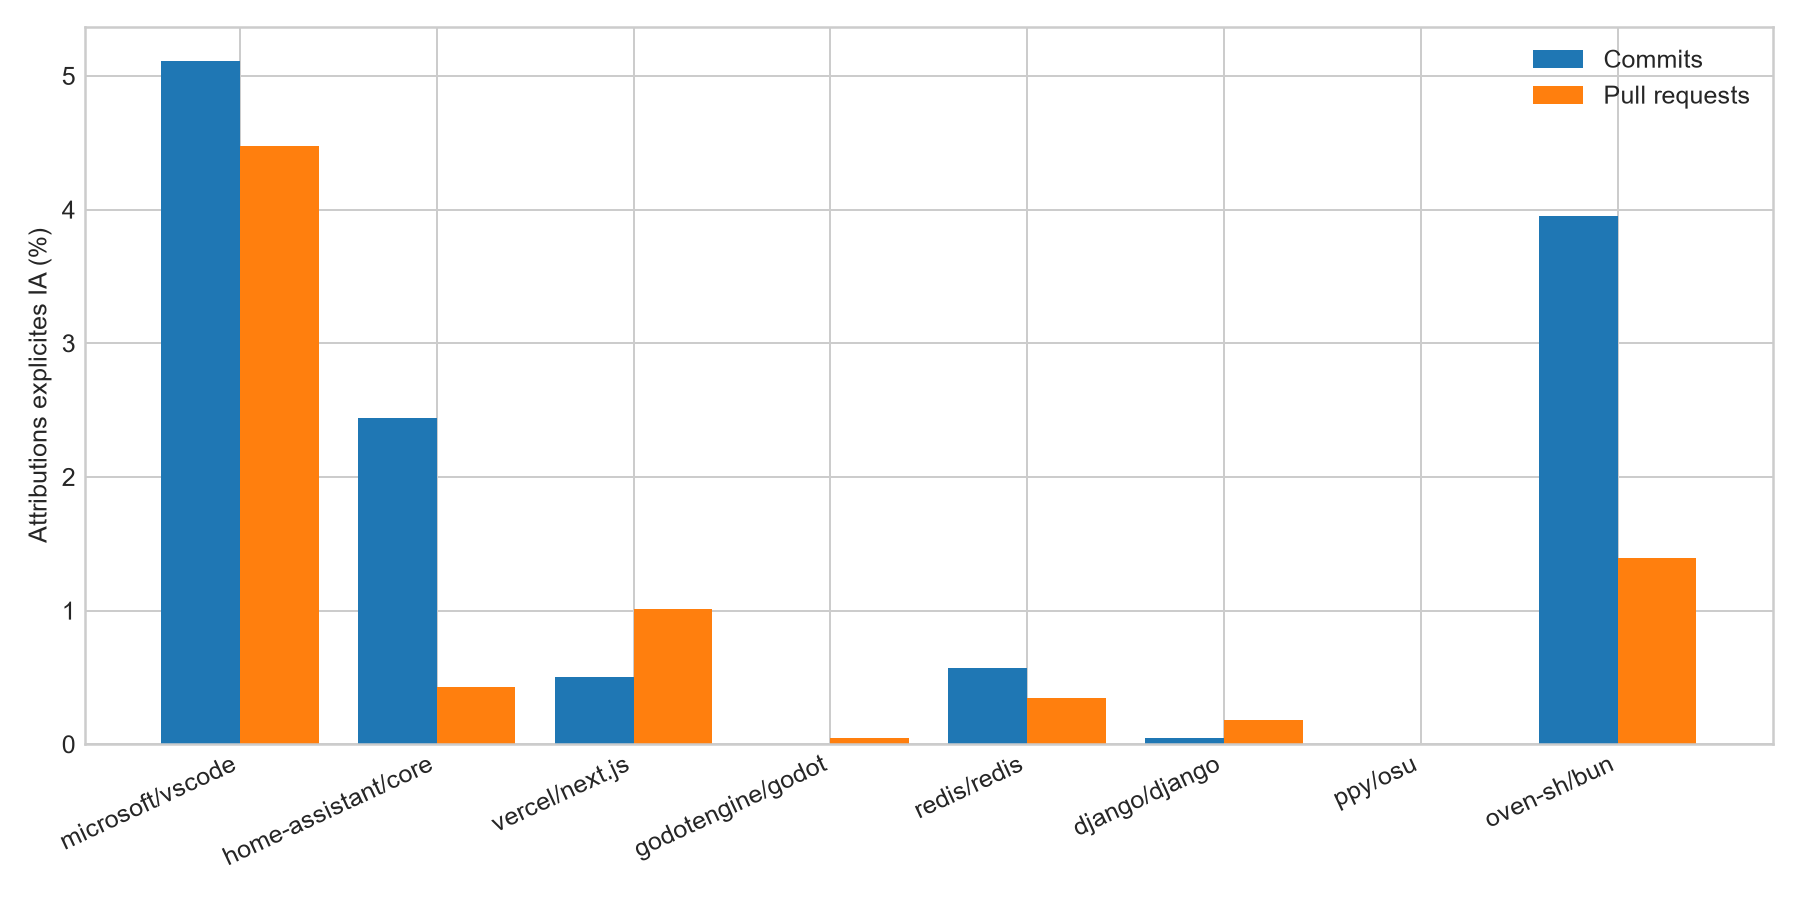
\includegraphics[width=\textwidth]{../Graphes_V2/taux_attribution_par_depot.png}
\caption{Taux d'attribution explicite par dépôt et par canal.}
\label{fig:taux}
\end{figure}

\section{Évolution temporelle}

La moyenne trimestrielle met en évidence une apparition tardive puis une progression des attributions visibles. Elle ne représente pas la proportion réelle de code produit par IA : elle mesure uniquement la fréquence des traces explicites parmi les pull requests.

\begin{figure}[H]
\centering
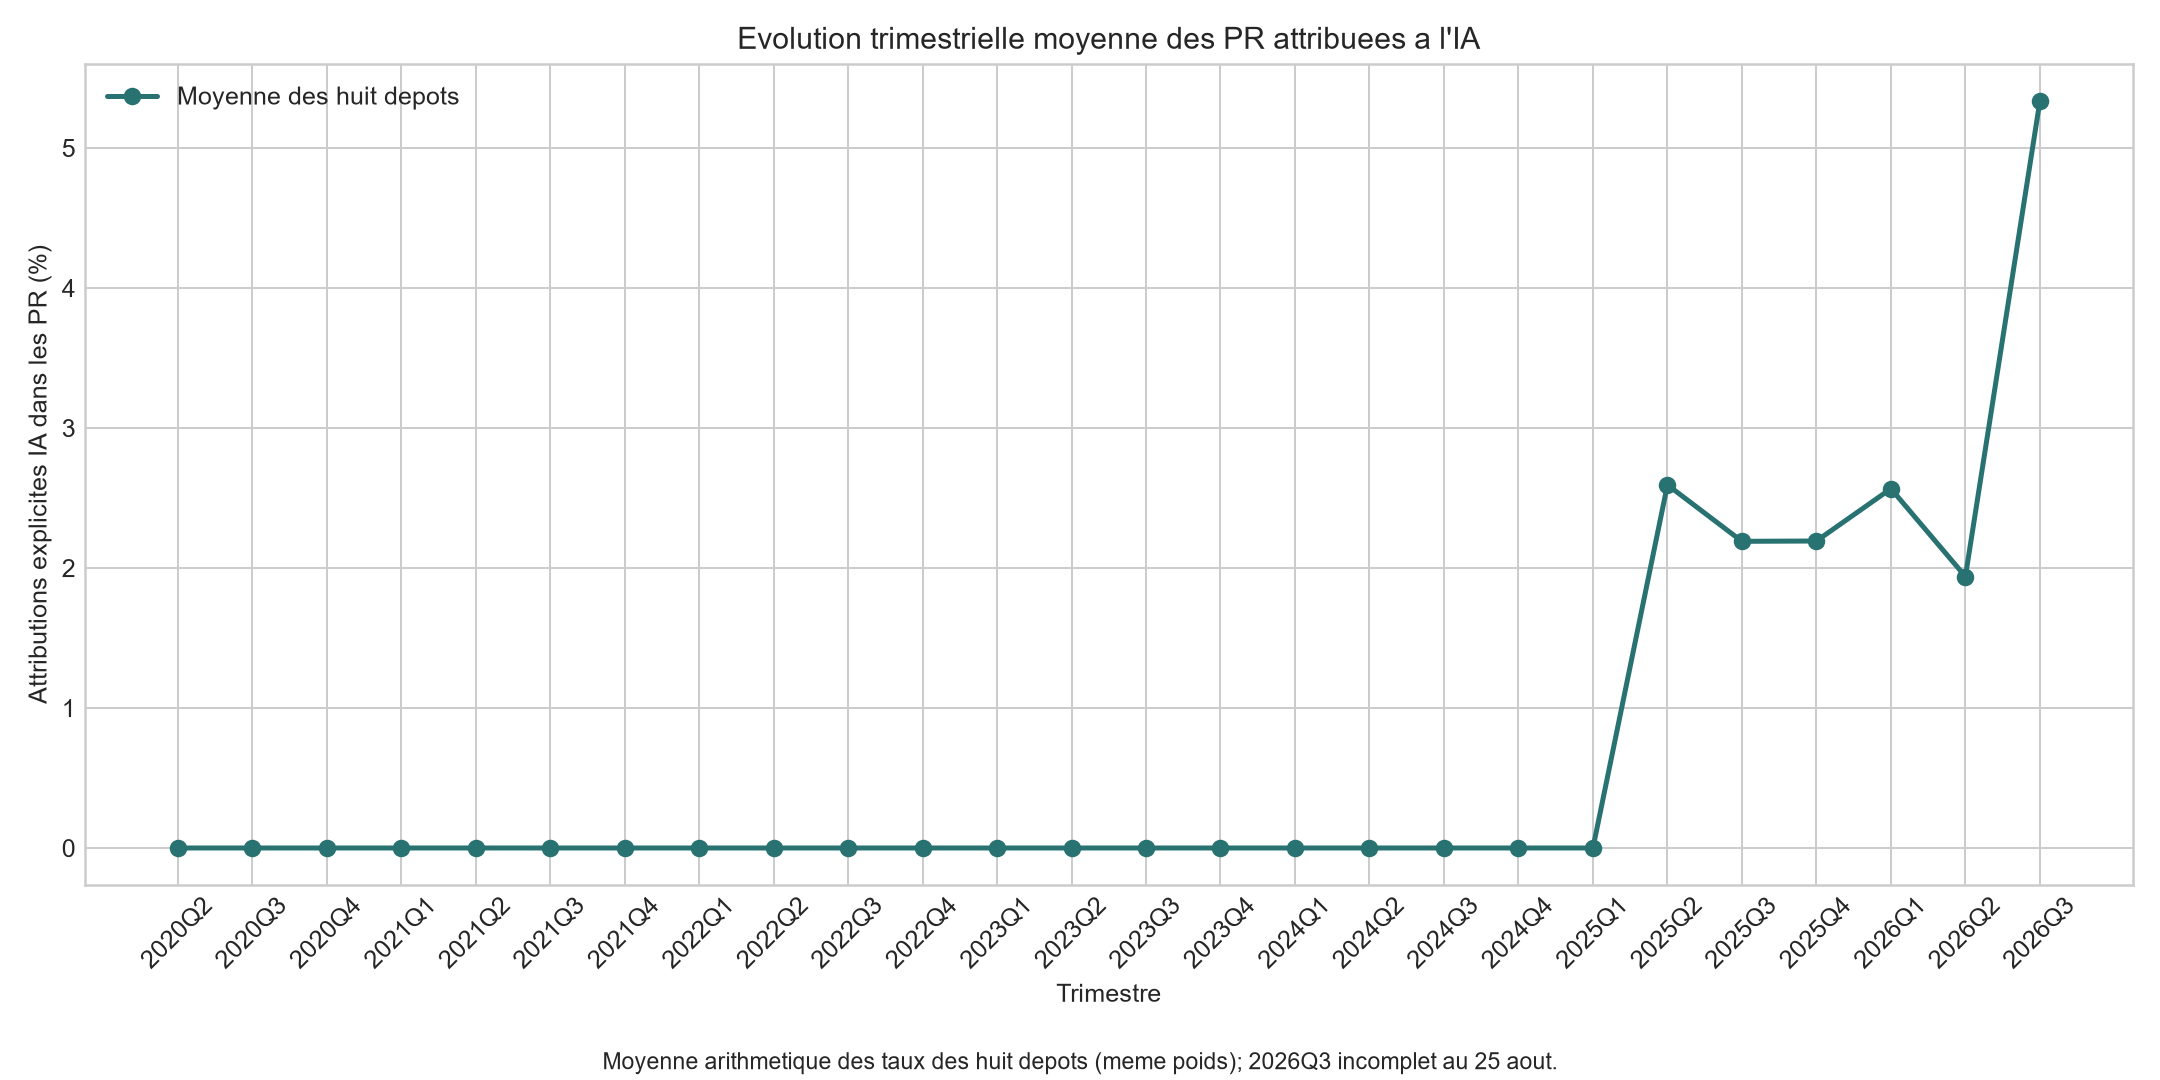
\includegraphics[width=\textwidth]{../Graphes_V2/evolution_trimestrielle_prs.png}
\caption{Évolution trimestrielle moyenne des pull requests explicitement attribuées à l'IA.}
\label{fig:evolution}
\end{figure}

La baisse apparente de Bun après 2025 doit être interprétée avec prudence. Les signaux auparavant visibles disparaissent alors que le nombre total de pull requests augmente. Il est impossible de savoir, à partir de ces seules données, si l'usage a réellement diminué ou si les outils et les conventions de déclaration ont changé.

\section{Comparaisons avant et après adoption}

Dans les trois dépôts où la date d'adoption est documentée, les taux augmentent après la bascule. Pour VS Code, le taux de pull requests attribuées passe de \taux{0,00} à \taux{8,85}. Pour Home Assistant, il passe de \taux{0,00} à \taux{1,48}. Pour Next.js, il passe de \taux{0,07} à \taux{6,74}. Les tests de Mann--Whitney appliqués aux taux trimestriels donnent respectivement $p=5{,}70\times10^{-5}$, $p=9{,}74\times10^{-6}$ et $p=2{,}20\times10^{-4}$.

Ces écarts vont dans le sens de H3 : lorsque l'usage est formalisé dans le dépôt, les agents deviennent plus visibles. La configuration n'est toutefois pas nécessairement la cause de cette hausse, et ces chiffres ne donnent aucune indication sur la qualité du travail produit.

\section{Validation externe du détecteur}

Sur AIDev, le rappel global V2 atteint \taux{95,18}. Il varie selon les outils : \taux{100} pour Devin, \taux{99,92} pour Google Jules, \taux{98,67} pour Copilot, \taux{95,21} pour Codex, \taux{93,60} pour Claude Code et \taux{87,19} pour Cursor. Cette différence s'explique notamment par la disponibilité inégale des identités de commit et des branches dans le corpus de référence.

\begin{figure}[H]
\centering
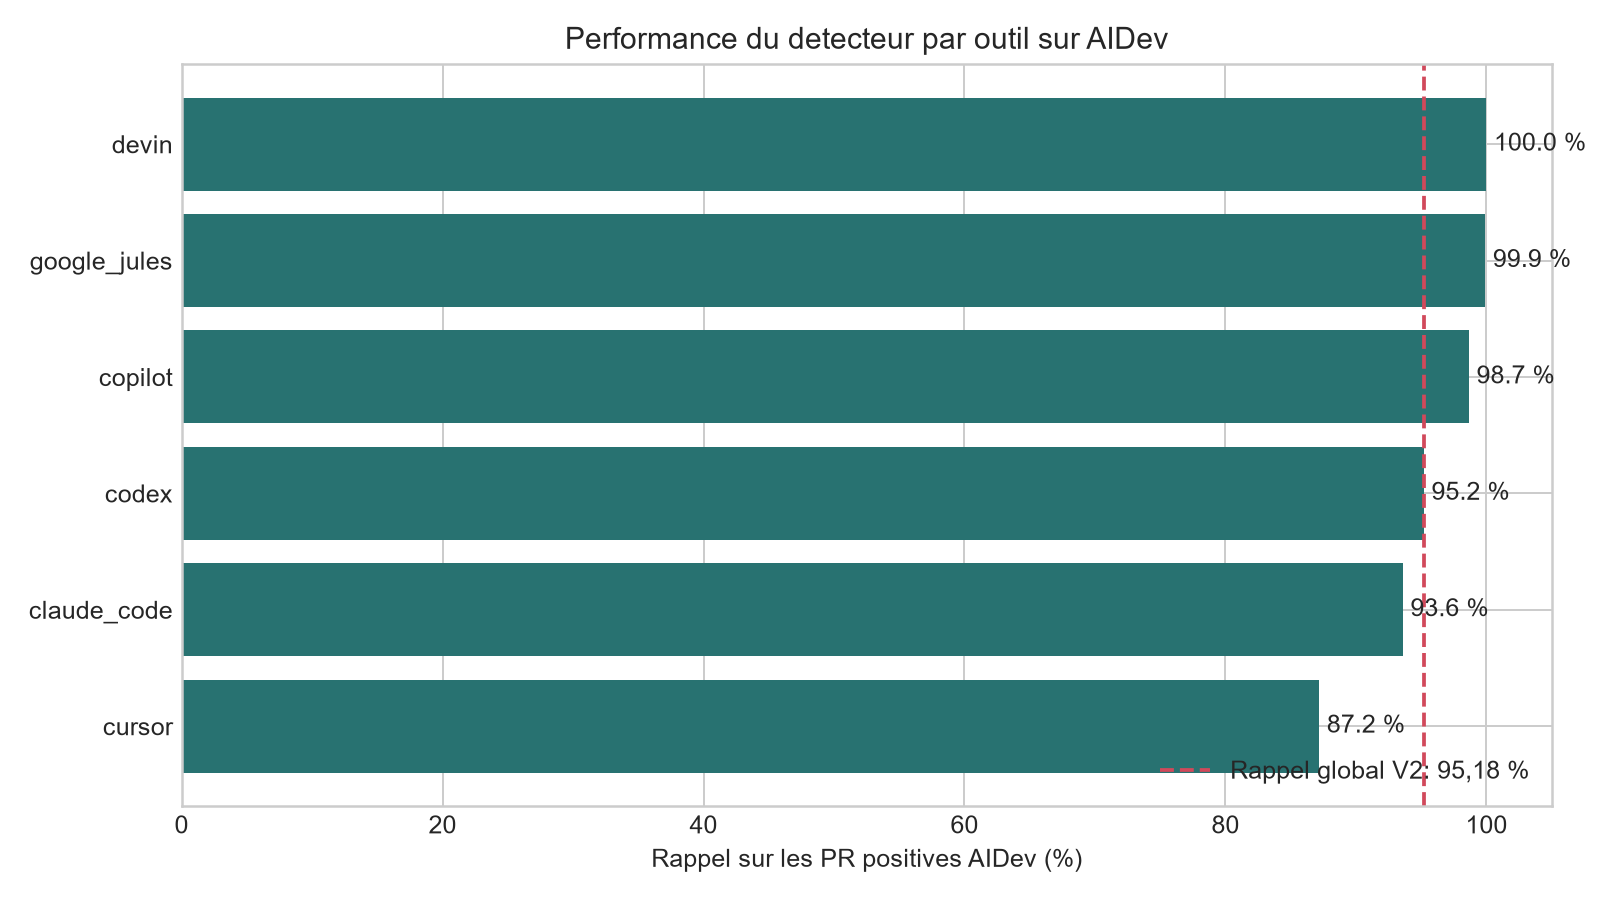
\includegraphics[width=0.9\textwidth]{../Graphes_V2/performance_aidev_par_outil.png}
\caption{Rappel du détecteur V2 par outil sur les cas positifs AIDev.}
\label{fig:aidev}
\end{figure}

La comparaison V1/V2 montre seulement six nouvelles détections dans les huit dépôts. La mise à jour améliore donc surtout la couverture externe sans bouleverser les résultats descriptifs du corpus principal.

\begin{figure}[H]
\centering
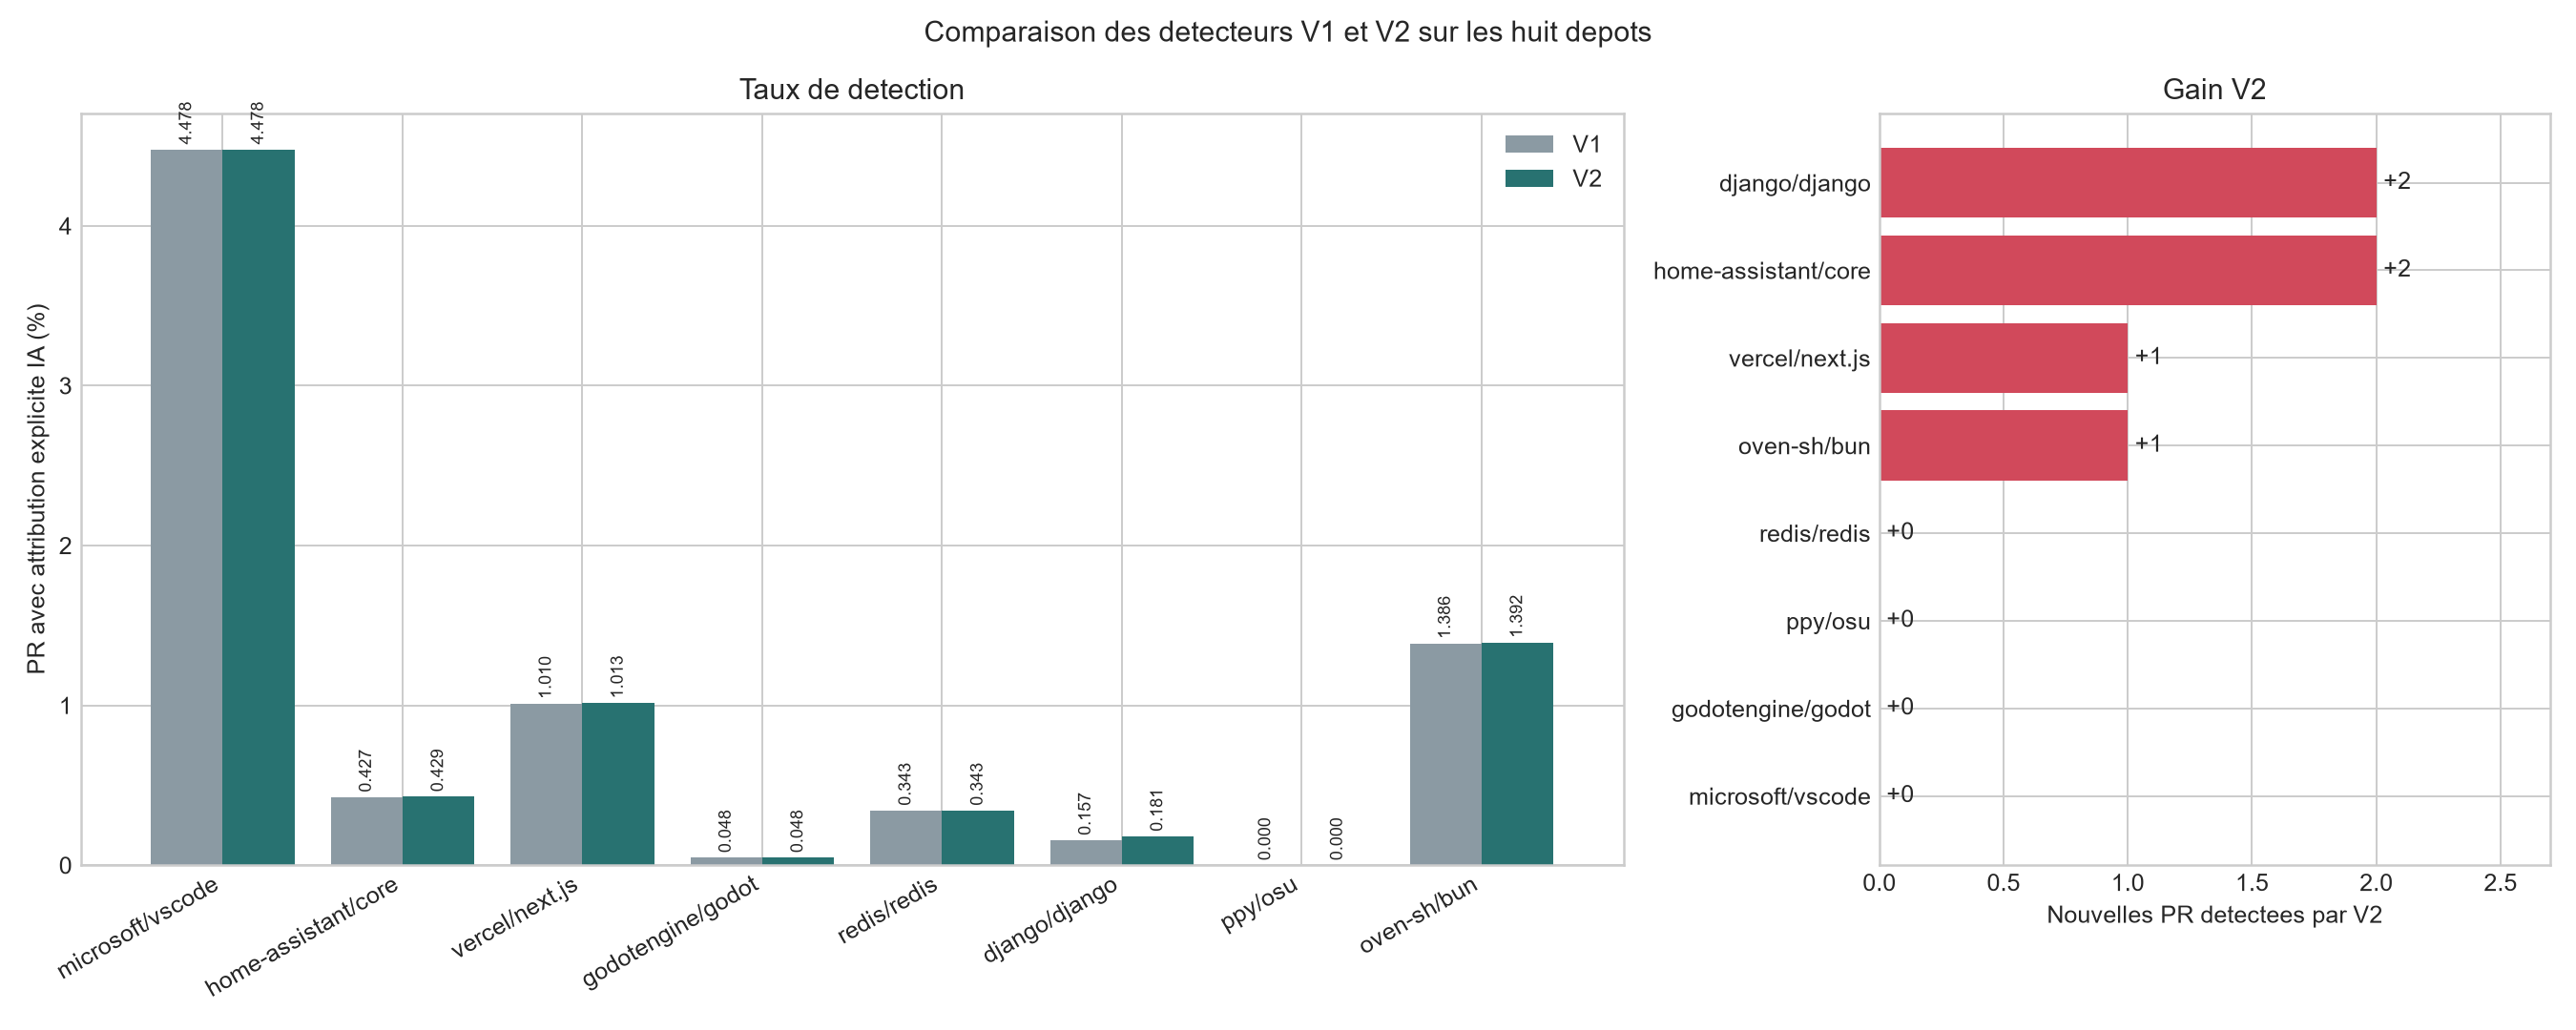
\includegraphics[width=\textwidth]{../Graphes_V2/comparaison_v1_v2_par_depot.png}
\caption{Comparaison des détecteurs V1 et V2 sur les huit dépôts.}
\label{fig:v1v2}
\end{figure}

\chapter{Discussion}

\section{Réponse à la question de recherche}

Les travaux étudiés ne décrivent pas un remplacement complet du développeur. Ils montrent plutôt un déplacement des activités. L'IA peut réduire le temps nécessaire pour obtenir une première solution, mais le développeur doit encore formuler le problème, choisir parmi les propositions, les vérifier puis les intégrer au travail de l'équipe.

Les résultats sur la productivité changent avec le contexte. \textcite{peng2023productivity} mesurent un gain important sur une tâche courte et autonome. \textcite{paradis2024enterprise} observent un gain plus modéré en entreprise. Chez des experts travaillant sur des dépôts qu'ils connaissent bien, \textcite{becker2025productivity} constatent au contraire un ralentissement. Il serait donc trompeur de résumer l'impact par une seule valeur moyenne.

Les outils produisent souvent du code fonctionnel, avec des résultats qui varient selon les tâches et les modèles. Les études de \textcite{pearce2022security} et de \textcite{fu2025weaknesses} trouvent des faiblesses de sécurité aussi bien dans des scénarios contrôlés que dans des extraits issus de GitHub. Une proposition générée doit donc être testée et relue comme n'importe quelle autre contribution.

Dans les dépôts étudiés, cette évolution laisse des traces concrètes : comptes dédiés, branches, messages de commit et pull requests. Leur fréquence augmente après les dates d'adoption retenues, mais varie fortement d'un projet à l'autre. Cette différence tient probablement autant aux règles de contribution qu'aux outils utilisés.

\section{Transformation des rôles et de la collaboration}

Avec un assistant, une partie du temps auparavant consacrée à l'écriture se reporte sur la revue. Le développeur choisit et corrige les propositions générées. Le relecteur, de son côté, doit s'assurer que la modification a réellement été comprise et contrôlée par la personne qui la soumet.

Dans les équipes, cette évolution peut déplacer le goulot d'étranglement de l'implémentation vers la revue. Une augmentation du nombre de pull requests n'est utile que si les tests, l'intégration continue et les relecteurs absorbent ce volume sans dégrader le niveau d'exigence. La performance locale d'un individu peut donc ne pas se traduire par une performance globale du collectif.

Les compétences attendues évoluent également. Savoir formuler une demande précise devient utile, mais ne remplace pas la compréhension du domaine, de l'architecture et des risques. Cette expertise aide à mieux cadrer l'outil et à écarter ses mauvaises propositions. On retrouve ici les modes d'accélération et d'exploration décrits par \textcite{barke2023grounded}.

\section{Conditions de réussite}

À partir de cette analyse, je retiens cinq conditions pour encadrer l'usage de ces outils :
\begin{enumerate}
  \item \textbf{Définir les usages autorisés.} Les données sensibles, les dépendances et les licences doivent être prises en compte avant l'adoption.
  \item \textbf{Maintenir une responsabilité humaine.} L'auteur de la modification reste responsable de sa compréhension et de sa validation.
  \item \textbf{Renforcer les contrôles.} Tests, analyse statique, revue de sécurité et intégration continue doivent accompagner l'augmentation de la production.
  \item \textbf{Mesurer plusieurs dimensions.} Temps de cycle, taux de défauts, retours en revue, maintenabilité et satisfaction doivent être observés conjointement.
  \item \textbf{Conserver la traçabilité.} Les déclarations explicites facilitent l'audit, l'évaluation et l'apprentissage collectif.
\end{enumerate}

\section{Limites}

Le détecteur observe les attributions explicites, pas l'origine réelle de chaque ligne. Les taux dépendent des pratiques de déclaration de chaque projet et constituent seulement une estimation minimale.

Les comparaisons avant/après ont aussi une portée limitée. Elles ne contrôlent pas toutes les évolutions dans le temps, et rien ne garantit que les dépôts de comparaison auraient suivi la même trajectoire. J'observe une association entre la date de bascule et la visibilité des agents, pas un effet causal sur la productivité ou la qualité.

L'évaluation sur AIDev porte uniquement sur des cas positifs. Elle mesure le rappel du détecteur, mais pas sa précision sur un ensemble indépendant. Il faudrait pour cela annoter manuellement un échantillon contenant à la fois des cas positifs et négatifs.

Une dernière difficulté vient de la vitesse à laquelle les outils évoluent. Les modèles, les interfaces et les pratiques de 2022 diffèrent déjà de ceux de 2025. Chaque résultat reste donc lié à une version de l'outil et à un protocole précis.

\chapter{Conclusion et perspectives}

Ce mémoire cherchait à comprendre l'impact de l'intelligence artificielle sur le développement logiciel. Les études examinées ne permettent pas de donner un chiffre unique. L'IA accélère certaines tâches et aide à explorer des solutions, mais elle ajoute aussi du temps de contrôle et peut donner confiance dans une réponse fragile.

Mon étude des dépôts apporte un autre constat : les agents laissent désormais des traces dans de grands projets publics. Les attributions explicites augmentent dans les dépôts qui ont formalisé leur adoption. Cette mesure ne dit pas combien de code est réellement produit par IA, mais elle montre que ces outils entrent progressivement dans le travail collectif.

Il n'existe donc pas de réponse unique à la problématique. L'IA transforme le développement en redistribuant le travail entre production et validation. Son bénéfice dépend de la tâche, de l'expertise, du contexte du dépôt et des règles mises en place par l'équipe. Elle peut augmenter la capacité de production, mais aussi accélérer la diffusion d'une erreur si les contrôles ne progressent pas au même rythme.

Pour prolonger ce travail, il faudrait d'abord constituer un échantillon annoté indépendant afin d'estimer la précision du détecteur. On pourrait ensuite relier les attributions au délai de fusion, au nombre d'itérations de revue, aux corrections, aux résultats des tests ou aux vulnérabilités. Des entretiens avec des développeurs compléteraient cette analyse en donnant accès à ce que les traces ne montrent pas : les stratégies de vérification, l'évolution des rôles et la manière dont chacun perçoit sa responsabilité.

\printbibliography[heading=bibintoc,title={Bibliographie}]

\end{document}